\chapter{Results}
\label{chap:results}



\noindent
Overall results summary

\section{Disparity} %Copied this in from the disparity paper

	When we compared tenrecs’ cranial morphologies to their closest relatives we found a trend towards higher disparity in tenrecs than
	in golden moles. However, these apparent differences were only
	significant for some disparity metrics. In contrast, golden moles have more diverse mandible shapes than tenrecs which appears to be due to greater morphological variety in the posterior mandible strucutres of golden moles (section \ref{sect:nonmic_gmoles}).

\subsection{\normalfont{Morphological disparity in tenrecs and golden moles}}
	Figures  \ref{fig:fourPCA} depict the morphospace plots derived from our principal components analyses of average Procrustes-superimposed shape coordinates for each species in our skull and mandible data respectively. We used the principal components axes which accounted for 95\% of the cumulative variation (n = 7, 8, 8 axes for the dorsal, ventral and lateral skull analyses respectively and n = 12 axes for the mandibles) to calculate the disparity of each family. 

%-----------------------------------------------------
%PCA figures: same one that's in the disparity paper
	%Source of this figure in my shape_data/output within the disparity folder 
	\begin{figure}[h]
	\centering
	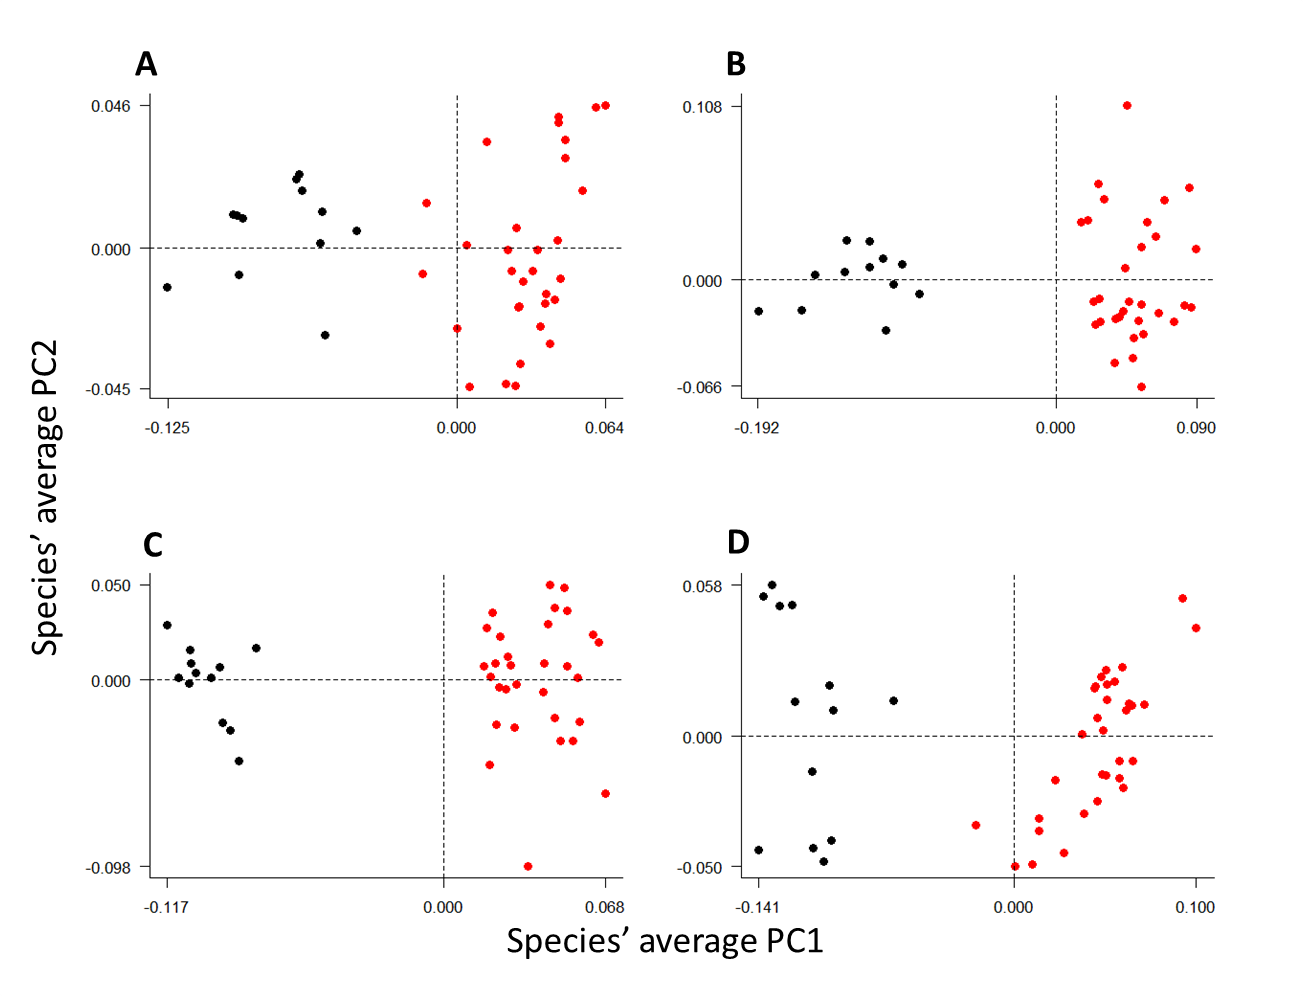
\includegraphics[width=1\linewidth]{Disparity/writing/figures/FourPlotPCA.png}
	\caption[Principal components plots of the morphospaces occupied by tenrecs and golden moles]
		{Principal components plots of the morphospaces occupied by tenrecs (red, n=31 species) and golden moles (black, n=12) for the skulls: dorsal (A), ventral (B), lateral (C) and mandibles (D) analyses. Axes are PC1 and PC2 of the average scores from a PCA analysis of mean Procrustes shape coordinates for each species. }
	\label{fig:fourPCA}
	\end{figure}
%--------------------------------------------------------

	Tenrecs and golden moles clearly have very different cranial and mandible morphologies: in each analysis, the families occupy significantly different areas of morphospace (npMANOVA, table \ref{tab:npmanova.summary}). 

%------------------------------------------------
%Summary table of the npMANOVA morphospace occupation comparisons	
	\begin{table}[!htb]	%!htb keeps the table within this section		

	\caption[Summary of npMANOVA comparisons of morphospace occupation for tenrecs and golden moles]
		{Summary of the npMANOVA comparisons of morphospace occupation for tenrecs and golden moles in each of the four analyses (three views of skulls and mandibles). In each case the two families occupy significantly different areas of morphospace.}
	\centering
	
%All tenrecs and golden moles
%npMANOVA results summary
%Values from the _manova.res files: npMANOVA based on the PC axes (not distance matrices)

\begin{tabular}[t]{l l l l }		
\hline
\textbf{Analysis} & \textbf{F} & R$^2$ & p value \\
\hline
Skulls dorsal & 66.02 & 0.62 & 0.001 \\
%-------------------------------------------
Skulls ventral & 100.74 & 0.71 &0.001 \\
%------------------------------------------
Skulls lateral & 75.07 & 0.65 & 0.001 \\
%------------------------------------
Mandibles & 59.34 & 0.59 & 0.001 \\
%-------------------------------------------------------
\hline
\end{tabular} 
	\label{tab:npmanova.summary}  
	\end{table}
%---------------------------------------
	Our comparisons of disparity levels within each family yielded different trends for the skulls compared to the mandible analyses.	
	In our analyses of the three different views of the skulls, when disparity is calculated from principal component - based metrics there is there is an overall trend for tenrecs to have higher disparity than golden moles. However, none of these differences are statistically significant (table \ref{tab:disp.summary}). In contrast, when we calculated disparity based on the sum of squared interlandmark differences between species pairs \citep{Zelditch2012} then golden moles had significantly higher levels of disparity than tenrecs (table \ref{tab:disp.summary}).

\bigskip
%------------------------------------------
%Summary table of the family comparisons for all tenrecs vs. golden moles
	\begin{table}[!htb]			
	\caption[Summary of disparity comparisons between tenrecs and golden moles]
		{Summary of disparity comparisons between tenrecs (T) and golden moles (G) for each of the data sets(rows) and five disparity metrics (columns). "Mandibles:one curve" refers to my shape analysis of mandibles excluding the three curves around the posterior structures of jaw (figure \ref{fig:sklat_landmarks}). Significant differences are highlighted in bold with the corresponding p value in brackets. Disparity metrics are; sum of variance, product of variance, sum of ranges, product of ranges and sum of squared distances among species. }
	\centering
	%Disparity family comparison results summary
%All tenrecs and golden moles
%Removed the SSqDist column because it was just making the whole paper more confusing (previous versions of the file include those results)

\begin{tabular}[t]{l l l l l  }		
\hline
\textbf{Disparity metric} & \textbf{SumVar} & \textbf{ProdVar} & \textbf{SumRange} & \textbf{ProdRange} \\
\hline
Skulls dorsal & T$>$G & T$>$G & T$>$G & T$>$G \\
%-----------------------------------------------------------
Skulls lateral	& T$>$G & T$>$G & T$>$G & T$>$G \\
%-------------------------------------------------------
Skulls ventral & T$>$G & G$>$T & T$>$G & T$>$G \\
%-------------------------------------------------------
Mandibles & G$>$T & \textbf{G$>$T* (0.008)} & \textbf{T$>$G* (0.025)} & \textbf{T$>$G* (0.009)}\\
%-------------------------------------------------------
Mandibles & G$>$T & G$>$T & T$>$G & T$>$G\\
%-------------------------------------------------------
\hline
\end{tabular} 
	\label{tab:disp.summary}  
	\end{table}
%------------------------------------------
\bigskip
	There is a less clear pattern from our analysis of disparity in the mandibles. Three of our five metrics indicate that golden moles have significantly higher disparity in the shape of their mandibles than tenrecs (table \ref{tab:disp.summary}) although one metric (sum of ranges) indicated the opposite result. 
	
	The three curves that we placed at the back of the mandibles (figure \ref{fig:mands_landmarks}) place a particular emphasis on shape variation in the posterior of the bone; the ramus, coronoid, condylar and angular processes. Therefore, higher disparity in golden mole mandibles compared to tenrecs could be driven by greater morphological variation in these structures. To test this idea, we repeated our morphometric analyses of the mandibles with a reduced data set of points; just the seven landmark points and one single curve at the base of the jaw between landmarks 1 and 7 (figure \ref{fig:mands_landmarks}). When we compared familial disparity levels with this reduced data set we found that golden moles no longer had significantly higher disparity than tenrecs but rather there were some indications that the opposite was true (table \ref{tab:disp.summary}).
	
\subsection{\normalfont{Morphological disparity in non-\textit{Microgale} tenrecs and golden moles}}
\label{sect:nonmic_gmoles} 	   
	
	We repeated our disparity comparisons with a subset of the tenrec specimens to remove the large and phenotypically similar \textit{Microgale} tenrec genus. In this case we found that tenrecs have significantly higher disparity than golden moles when the skulls are analysed in lateral view (table \ref{tab:disp.nonmic.summary}). However, none of the other comparisons in any of the analyses were significant. Similarly, the trend in the main analysis for golden moles to have significantly higher disparity measured as the sum of squared inter-landmark distances (table \ref{tab:disp.summary}) was not repeated in this comparison of disparity in non-\textit{Microgale} tenrecs and golden moles (table \ref{tab:disp.nonmic.summary}).
\bigskip
%-------------------------------------------------------
%Summary of the family comparisons for non-Microgale tenrecs vs. golden moles
	\begin{table}[!htb]			
	\caption[Summary of disparity comparisons between non-\textit{Microgale} tenrecs and golden moles]
		{Summary of disparity comparisons between non-\textit{Microgale} tenrecs (T) and golden moles (G) for each of the data sets(rows) and five disparity metrics (columns). Significant differences are highlighted in bold with the corresponding p value in brackets. Disparity metrics are; sum of variance, product of variance, sum of ranges, product of ranges and sum of squared distances among species. }
	\centering
	%Disparity family comparison results summary
%Non-Microgale tenrecs and golden moles

%Removed the SSqDist metrics from the paper because they were just causing confusion

\begin{tabular}[t]{l l l l l }		
\hline
\textbf{Disparity metric} & \textbf{SumVar} & \textbf{ProdVar} & \textbf{SumRange} & \textbf{ProdRange} \\
\hline
Skulls dorsal & T$>$G & T$>$G & T$>$G & T$>$G\\
%-----------------------------------------------------------
Skulls lateral	& \textbf{T$>$G* (0.014)} & T$>$G & \textbf{T$>$G* (0.001)} & \textbf{T$>$G*(0.003)}\\
%-------------------------------------------------------
Skulls ventral & T$>$G & T$>$G & T$>$G & T$>$G\\
%-------------------------------------------------------
Mandibles & T$>$G & G$>$T & T$>$G & G$>$T\\
%-------------------------------------------------------
%Don't need to do a subset analysis of mandibles for non-Microgale tenrecs
%Mandibles one curve & G$>$T & T$>$G & T$>$G & T$>$G & G$>$T\\
%-------------------------------------------------------
\hline
\end{tabular} 
	\label{tab:disp.nonmic.summary}  
	\end{table}
%------------------------------------	


%**********************************************

\section{Convergence}





